\documentclass[12pt]{article}

\usepackage[margin=1in]{geometry} % 1-inch margins
\usepackage{times}                % Times (Times New Roman–like) font
\usepackage{fancyhdr}             % For custom headers/footers
\usepackage{setspace}             % For spacing
\usepackage{titlesec}             % For section formatting
\usepackage{enumitem}             % For list alignment
\usepackage{graphicx}             % For image insertion
\usepackage{caption}

\pagestyle{fancy}
\fancyhf{} % Clear default header and footer

% Header on the right side
\fancyhead[R]{Saksham AI: Multilingual Virtual Interviewer}

% Footer on the left side
\fancyfoot[L]{Pillai HOC College of Engineering \& Technology (Autonomous), Rasayani}
\fancyfoot[R]{\thepage} % Ensure page number is displayed on the right footer

% Horizontal lines in header & footer
\renewcommand{\headrulewidth}{0.4pt} 
\renewcommand{\footrulewidth}{0.4pt} 

% Set the page number to start from 25
\setcounter{page}{27}

% Paragraph Formatting
\setlength{\parindent}{1.5em} % Indent first line
\setlength{\parskip}{0em}     % No extra space between paragraphs
\onehalfspacing               

\begin{document}

\vspace*{\fill}

\begin{center}
    {\Large \bf Chapter 6} \\[2em] % Line break with extra space (1em)
    {\Large \bf Project Design}
\end{center}
\vspace*{\fill}

\newpage

% Set section counter to 6 so that it starts as Chapter 6
\setcounter{section}{6}

\newpage

% SECTION 6.1: DATA FLOW DIAGRAM
\subsection{Data Flow Diagram}
\vspace{10pt}

DFD (Data Flow Diagram) is a graphical representation of a system or process, which shows
how data flows through various components of the system. It represents the flow of data within the system and between its different components.

\vspace{1em}

% SUBSECTION 6.1.1: DFD Level 0
\subsubsection{DFD Level 0}
\vspace{10pt}

\noindent DFD (Data Flow Diagram) is a graphical representation of a system or process, which shows how data flows through various components of the system. It is the way of representing the flow of data within a system and between its different components.\\
DFD Level 0 is also called a context diagram. It's a basic overview of the whole system or process being analyzed or modelled. It's designed to be an at-a-glance view, showing the system as a single high-level process, with its relationship to external entities. DFD level O data flow from user to the system. The work of user initialization, result and final report is executed.


\vspace{10pt}

\begin{center}
    \fbox{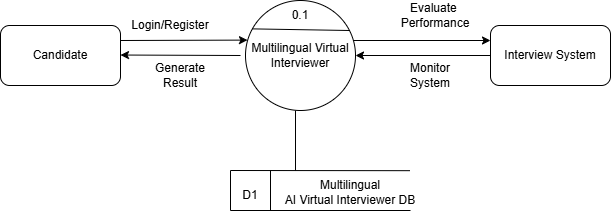
\includegraphics[width=1.0\textwidth]{dfd1.png}}
\end{center}

\begin{center}
    Figure 6.1.1: DFD Level 0
\end{center}
\noindent The Fig. 6.1.1 illustrates the Level-0 Data Flow Diagram of the Multilingual Virtual Interviewer system, where the entire platform is represented as a single processing unit. The diagram shows how data flows between the candidate and the system during different stages of the interview process. The candidate interacts with the system by providing inputs such as registration details, login credentials, interview responses, and requests to view results. The system verifies and processes this information to authenticate the candidate and initiate the interview session.






\vspace{20pt}
\newpage
% SUBSECTION 6.1.2: DFD Level 1
\subsubsection{DFD Level 1}
\vspace{10pt}

\noindent A Level 1 Data Flow Diagram (DFD) provides a detailed breakdown of the main processes involved in the Multilingual Virtual Interviewer system. It represents an exploded view of the context diagram, showing how data flows from the candidate through various internal modules of the system. The above figure illustrates the Level 1 DFD detailing the specific data exchanged between the external entity (Candidate) and the internal sub-processes of the platform. Information such as credentials, interview responses, translated content, and evaluation results is exchanged during different stages of operation:



\vspace{10pt}

\begin{center}
    \setlength{\fboxrule}{1pt}  % Border thickness
    \setlength{\fboxsep}{5pt} 
    \fbox{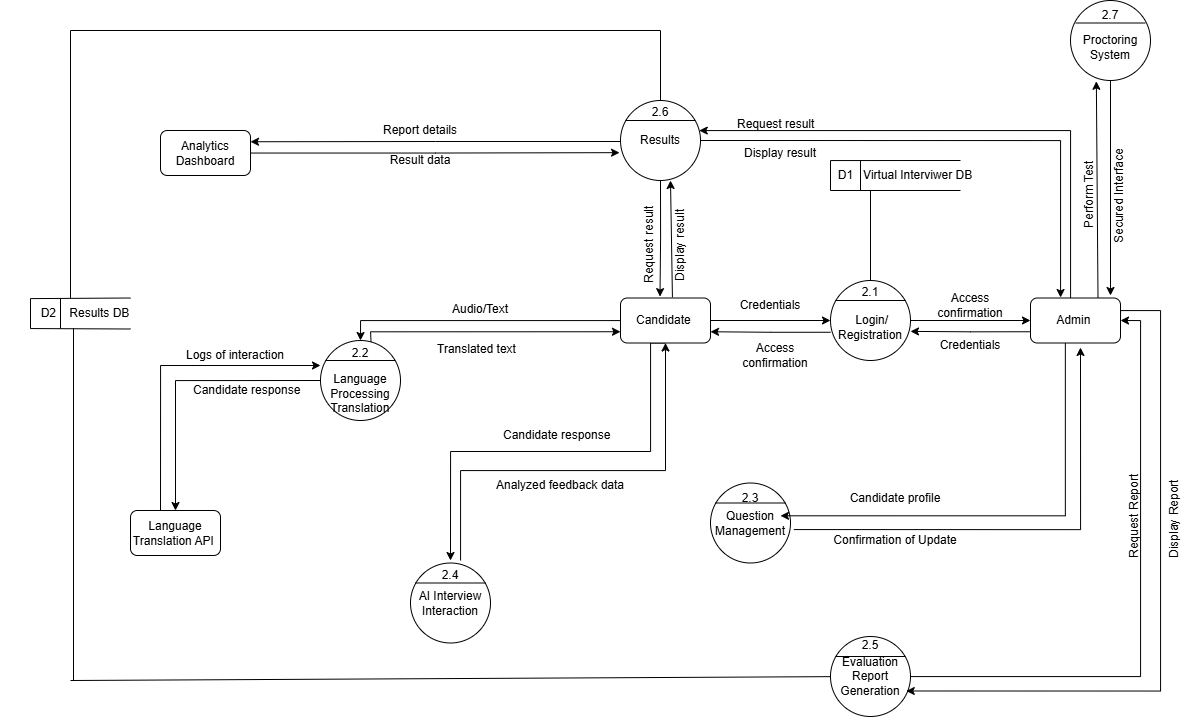
\includegraphics[width=1.0\textwidth, keepaspectratio]{dfd2.png}}
\end{center}
\begin{center}
    Figure 6.1.2: DFD Level 1
\end{center}

\noindent The Fig. 6.1.2 illustrates the Level-1 Data Flow Diagram of the Multilingual Virtual Interviewer system, showing the detailed internal working of the interview process. The interaction begins when the candidate performs login or registration by providing credentials through the user interface. The system verifies these details with the Virtual Interviewer database and grants access upon successful authentication. Once logged in, the candidate starts the interview session and submits responses in audio or text form. These responses are forwarded to the language processing module, where speech-to-text conversion, translation, and linguistic analysis are performed to support multilingual interaction.



% SUBSECTION 6.1.1: DFD Level 2
\subsubsection{DFD Level 2}
\vspace{10pt}

\noindent A Level 2 Data Flow Diagram (DFD) provides a more detailed decomposition of the processes presented in the Level 1 DFD of the Multilingual Virtual Interviewer system. It breaks down each major function, such as authentication, interview interaction, language processing, AI evaluation, and result generation, into smaller sub-processes to clearly illustrate how data is handled internally. This level shows the step-by-step flow of candidate inputs, system processing, database interactions, and output generation.
\vspace{5pt}

\begin{center}
    \fbox{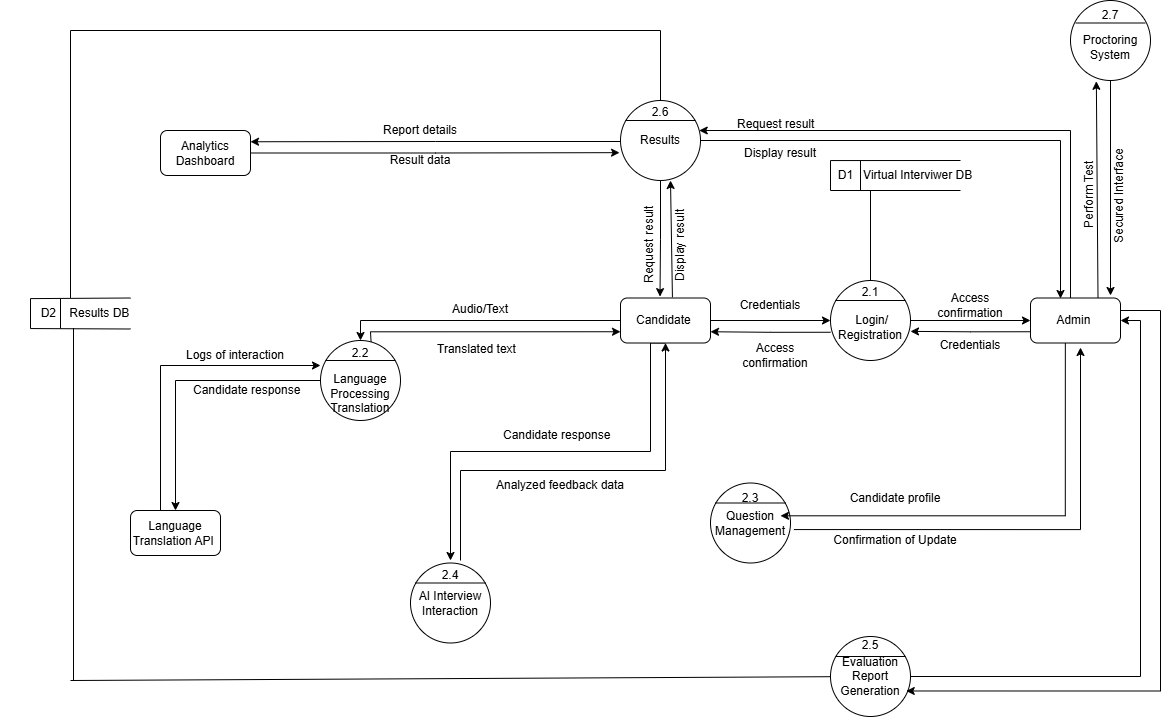
\includegraphics[width=1.0\textwidth]{dfd3.png}}
\end{center}

\begin{center}
    Figure 6.1.3: DFD Level 2
\end{center}
\noindent The Fig. 6.1.3 illustrates the Level-2 Data Flow Diagram of the Multilingual Virtual Interviewer system, presenting a detailed breakdown of internal sub-processes and data interactions during the interview workflow. The process begins with the candidate performing login or registration by submitting credentials, which are verified against the Virtual Interviewer database to grant secure access. Once authenticated, the candidate participates in the interview by providing responses in audio or text form. These inputs are forwarded to the language processing module, where speech-to-text conversion, translation, and linguistic analysis are performed to support multilingual communication.


\vspace{20pt}
\newpage

% SECTION 6.2: FLOW CHART
\subsection{Flow Chart}

\vspace{15pt}

\noindent The Fig. 6.2 illustrates the flowchart of the Multilingual Virtual Interviewer system, describing the step-by-step operation of the interview process. The workflow begins when the candidate enters personal details and selects a preferred language for the interview session. Based on this information, the system generates an appropriate interview question and translates it into the chosen language for better understanding. The candidate then provides a response either through voice input or direct text entry. If voice input is used, the system converts the speech into text using a speech-to-text module before further processing. Both voice-derived text and directly entered text responses are then translated into the system’s internal language to ensure uniform evaluation.After translation, the response is forwarded to the AI evaluation engine, which analyzes the content based on predefined criteria such as relevance, clarity, technical correctness, and communication effectiveness. The system subsequently displays an immediate score along with constructive feedback to the candidate. Following this, the system checks whether additional questions are required to complete the interview session. If more questions remain, the workflow loops back to the question generation stage and repeats the process for the next question. If no further questions are pending, the system compiles the overall performance metrics to generate the final result report. Finally, the consolidated evaluation, including scores, feedback, and performance insights, is presented to the recruiter for decision-making purposes.



\begin{figure}[h]
    \centering
    \setlength{\fboxrule}{1pt} % Border thickness
    \setlength{\fboxsep}{0pt} % Space between image and border
    \renewcommand{\thefigure}{6.2} % Manual figure number
    \fbox{\includegraphics[width=0.4\textwidth]{flowchart.png}}
    \captionsetup{labelformat=empty} % Remove default "Figure X.Y:"
    \caption{Figure \thefigure: Flow Chart Representation }
\end{figure}

\end{document}
